%----------------------------------------------------------------------------------------
%	GRADE TABLES
%----------------------------------------------------------------------------------------

\par{\centering\Large \hypertarget{grds_ms}{Master of Science in \textsc{Computer Science}}\par}
\large{\centering Grades\par}\normalsize

\begin{center}
\begin{tabular}{lcc}
\multicolumn{1}{c}{\textsc{Course}} & \textsc{Grade}&\textsc{Credit Hrs}\\
\hline
Final Internship                                           &       77,5/100 & 18    \\
Research Group : Distributed Applications                  &       70/100 & 3     \\
Research Group : Informatics Systems                       &       85/100 & 3     \\
Engineering Group : Embedded Systems                       &   80/100 & 3     \\
Engineering Group : Distributed Systems                    &     62,5/100   & 3     \\
\hline
Advanced Distributed Algorithms                            &  75,1/100 & 3     \\
Advanced Parallel Programming                              &    87/100 & 3     \\
Automated Production of Distributed Applications           &  72,5/100 & 3     \\
Formal Verification of Distributed Systems                 &  67,5/100 & 3     \\
Mobile Device Programming                                  &  62,1/100 & 3     \\
Foundation of Real-Time Embedded Systems                   &   100/100 & 3     \\
Platforms for Advanced Informatics Systems                 &  75,1/100 & 3     \\
Parallel Programming                                       &    77/100 & 3     \\
Multi-core Kernels and Virtualization                      &  88,5/100 & 3     \\
Environments for Embedded or Real-Time Distributed Systems &  67,5/100 & 3     \\
\hline
Project : Kernel Placement Algorithm                       & 93,75/100 & 6     \\
Distributed Databases                                      & 83,85/100 & 6     \\
Distributed Algorithms                                     &    67/100 & 6     \\
English                                                    & 79,25/100 & 6     \\
Client/Server Distributed Systems                          &  95,1/100 & 6     \\
Networks and System Administration                         &  91,5/100 & 6 \\
\hline
OS Kernel's Advanced Architecture                          &  89,5/100 & 6     \\
Processor's Architecture and Optimisations                 &    54/100 & 6     \\
POSIX Advanced Programming                                 &  70,5/100 & 6     \\
Software Engineering                                       &    82/100 & 6     \\
Networks' Architecture	                                   &    64/100 & 6     \\
Advanced Algorithmic                                       &    85/100 & 6 \\
\hline
\end{tabular}
%{\footnotesize N/A* Not yet available}
\end{center}
\bigskip
\bigskip

%------------------------------------------------

\newpage

\par{\centering\Large \hypertarget{grds_bs}{Bachelor of Science in \textsc{Computer Science and Applied Mathematics}}\par}\large{\centering Grades\par}\normalsize

\begin{center}
\begin{tabular}{lcc}
\multicolumn{1}{c}{\textsc{Course}} & \textsc{Grade} & \textsc{Grade Points}\\
\hline
\textsc{2011 - 2012} & & \\
\hline
Introduction to Numerical Imaging                          &  77,5/100 & 6     \\
Introduction to Cryptology                                 &   100/100 & 6     \\
Models for Optimization and Decision                       &  62,5/100 & 6     \\
Numerical Methods for differential equations               & 65,94/100 & 6     \\
Bioinformatics                                             &    65/100 & 3     \\
English                                                    &    71/100 & 3     \\
\hline
Object-oriented Programming                                &  87,5/100 & 6     \\
Algorithm Analysis and Conception                          & 80,63/100 & 6     \\
Introduction to Numerical Analysis                         &    49/100 & 6     \\
Probability                                                &    67/100 & 6     \\
Introduction to Topology and Calculus                      &    88/100 & 6     \\
English                                                    &  72,5/100 & 3     \\
\hline
\textsc{2010 - 2011} & & \\
\hline
Brown Exchange : Introduction to Machine Learning          &    70/100 & 6     \\
Analysis and Algebra                                       &    77/100 & 3     \\
Multi-variable functions and multi-integrals               & 85,25/100 & 6     \\
English                                                    &    84/100 & 3     \\
\hline
Geometry and Algebra                                       &    53/100 & 12    \\
Introduction to System multiprogramming                    &  82,1/100 & 6     \\
Scientific Computation                                     &    70/100 & 6     \\
Algorithmic                                                &  72,5/100 & 6     \\
\hline
Imperative Programming and Data Structure in C             & 90,74/100 & 6     \\
Introduction to Tasks Automation                           & 58,88/100 & 6     \\
Arithmetic                                                 &    63/100 & 6     \\
Series and Integrals                                       &  65,5/100 & 12    \\
\hline
\end{tabular}
\end{center}

%----------------------------------------------------------------------------------------

\newpage

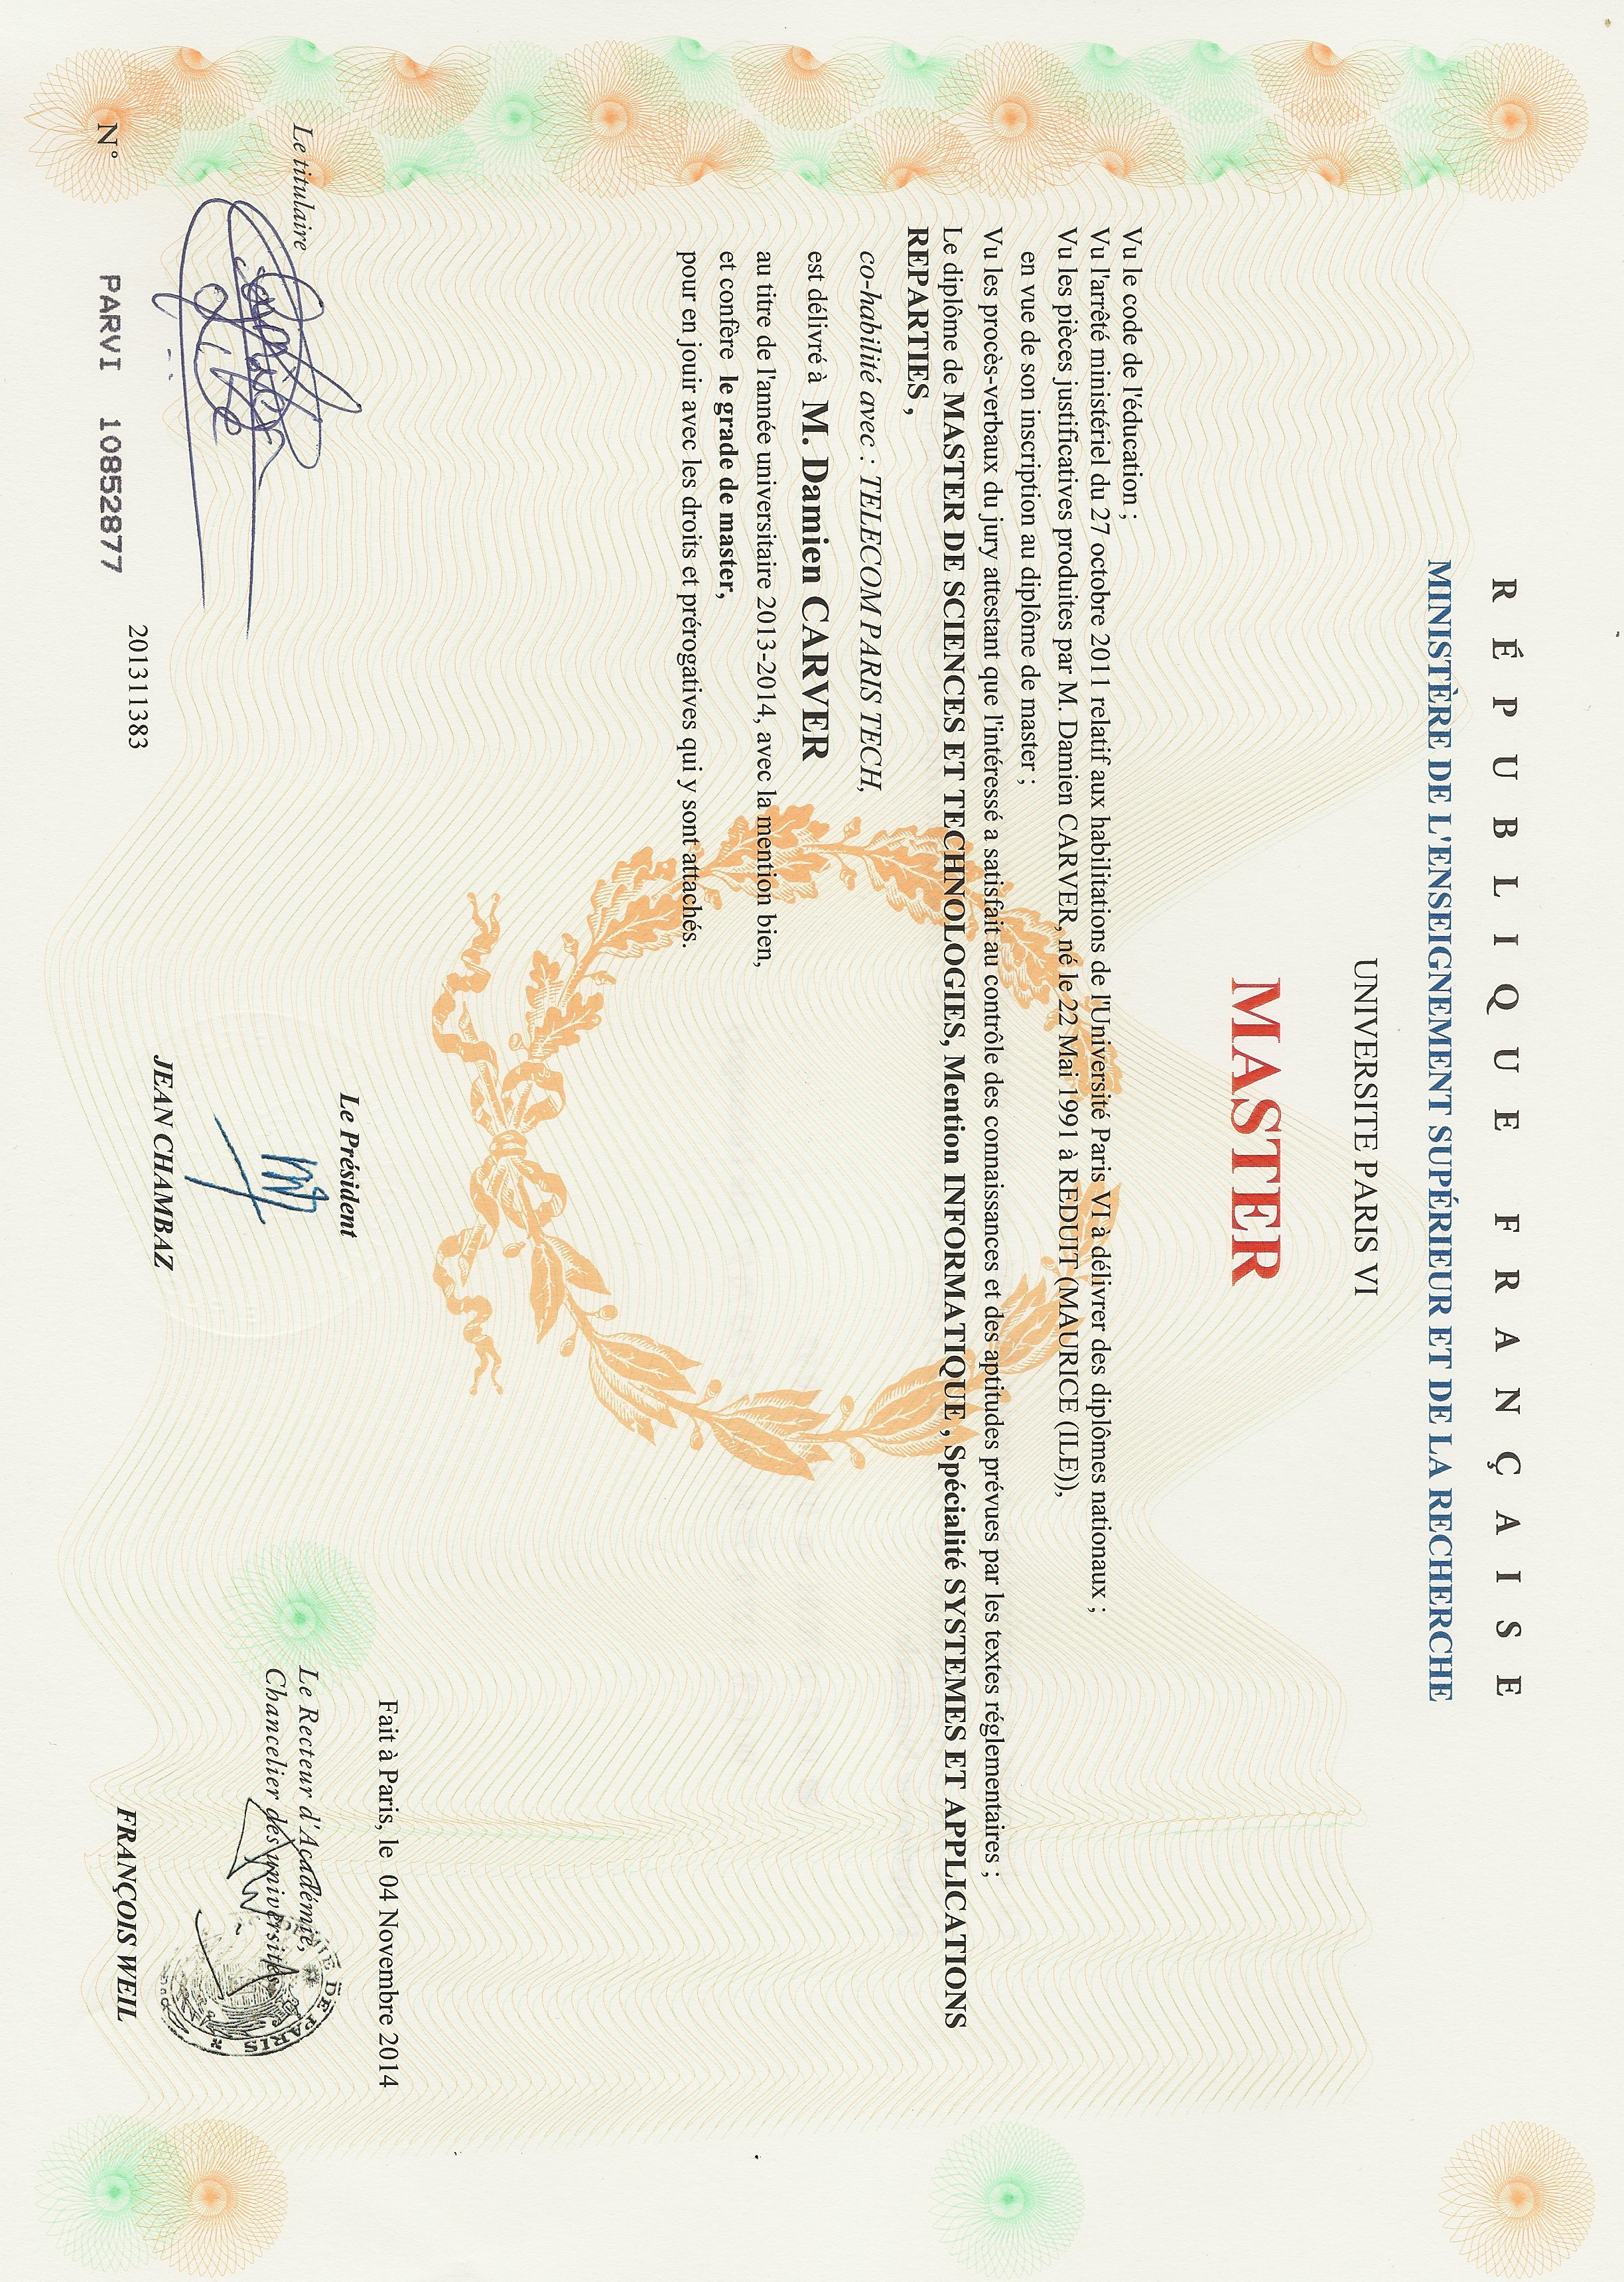
\includegraphics[scale=0.7]{./m2.jpeg}

%----------------------------------------------------------------------------------------